\chapter{Background}

\section{Recommendation Systems}
\subsection{Problem Statement}
Generally speaking recommendation systems are concerned with recommending items to be of use to users.
The recommendations should help the users decide which items to buy, music to listen to, what news articles to read etc.
Virtually any decision-process can be made easier for users by providing recommendations.
Typically recommendation systems are used by online services, famously for example by Spotify for music~\cite{rec_spotify} and YouTube for videos~\cite{rec_yt}.
By using these online service the users generate data that the service can use to improve the recommendations, for example rating videos gives the operator of the service a datapoint on how much a video is liked by a specific user.
However also retailers are known to use recommendation systems, based on data generated by customer loyalty programs such as Migros Cumulus~\cite{rec_migros} retailers tailor coupons or other offers to their customers.
In principle data of users interacting with items (viewing, buying, rating etc.) serves as the basis for a recommendation system. 
Depending on the use-case this data is utilized to assign scores to items depending on the user. 
The semantic meaning of a score depends on the objective of a recommendation system.
For example a system which recommends products to be bought might assign a "probability of purchase", whereas a system which recommends videos might predict the probability of a user watching a video to the end. 
\\
Bringing this all together we can define a general recommendation system with the following function:
\begin{equation}\label{eq:recommendation_system}
    s = f(i, u, h_u)
\end{equation}
Where $s$ is the assigned score to item $i$ for the user $u$ and the users history $u_h$. 
The users history represents all the previous interactions with items.
Essentially when we design a recommendation engine we want to learn the function $f$.
To assess the quality of the learned function we need to know the "true" score for the specific item and user, this can be done in different ways.
Usually during training we will hold off later interactions with items, and test the learned functions on those.
However as soon as the users sees recommendations, we essentially change the reality, i.e. we don't know what the user saw as recommendations, if any, in the user history, therefore it makes sense to also assess the performance of a recommendation engine in production.
\subsection{Properties of Recommendation Systems}
In the following we will look at different properties of recommendation systems.
Typically recommendation systems have a combination of the following properties.
\paragraph{User-based}
User-based recommendation system base the information used to make recommendations mainly on properties of the user, such as gender, age, etc.
Also information from the history of the user can be used, for example what the user has bought or read before.
Essentially that means when we try to generate recommendations for a specific user we try to find similar users and recommend items that the similar users liked. 
\paragraph{Item-based}
Item-based recommendation system use mostly information about the item to produce recommendations, such as item type (e.g. genre of a movie).
However as the name suggests, the basis for a recommendation is always a specific item, for example a product a user is looking at online.
This item the user is currently interacting with is referred to as the "active item". 
Usually item-based recommendation systems then try to find similar items to the currently active item. 
The method of finding similar items can be arbitrarily complex, identifying similar items is its own field of research.
What is also often done is combine this approach with a user-based component, where the similar items are sorted or filtered based on the user.
An example of this might be the following:
\begin{itemize}
    \item Steve is a male looking at black shirts.
    \item When extracting similar products we find a range of black shirts, also containing womens shirts.
    \item If we would recommend items by popularity the womens shirts would appear as the first recommendation, since women typically buy more shirts.
    \item Instead of directly displaying the recommendations we filter out the womens shirts that is found in this selection.
\end{itemize}
\paragraph{Session-based}
Session-based recommendation systems are a rather new form of such a system.
A session is a sequence of interactions from a user with one or several items.
Depending on the use-case and setting this can be defined differently.
Usually online-services define a session as the sequence of interactions a user produces on the site until closing the browser window.
Obviously sessions can have variable lengths, therefore it is difficult to directly feed that information into a recommendation system.
However with the rise of Recurrent Neural Networks (c.f.~\ref{rnn}) a powerful tool for handling variable length sequence data becomes available.
Session-based recommendation systems use RNNs to model the sequence data generated by sessions to achieve two things.
First by using RNNs we can extract a fixed dimensional representation of a specific session, this allows us to compare different sessions.
Second by using the fixed representation of a session we can try to identify the intent a user has in a specific session, based on this recommendations can be made to fulfill the users intent.
An intent can be defined as the goal the user has in a specific session.
In the example of an online-shop there are a few different, well-known intents identified by analysts such as: Browsing for inspiration, searching for a specific product, buying a specific product, researching products etc.
Also these intents exist in different contexts, in the case of an online-shop the contexts can be different product types (mobile phone, couch, dining table) etc.
From the above explanation it is intuitive to see why these systems are more desired by operators of online services, since the recommendations can be targeted much more specific to the user and his intent, instead of just general information of the user and the active item. 
\paragraph{Collaborative}
Collaborative recommendation-systems mostly use interaction data to generate recommendations.
For example we use the clicks on products as a data source and then predict which products the user will click next.
However the collaborative aspect comes from the fact that we source other users interactions as a basis for the recommendations.
In principle we view different users as versions of possible behaviour of a user, the more interactions two users have in common, the more similar they are assumed to be.
Therefore we can extend the behaviour (i.e. product views) of a user by looking at what similar users have done on the same active item.
\paragraph{Content-based}
In contrast to collaborative recommendation systems, content-based systems heavily rely on so called content information.
Content information refers to the actual content of different items.
The name stems from early recommendation systems which mainly focussed on recommending media.
The idea is to actually analyze the content of an item, be it the images in a movie, the soundwaves of a song or the text in a book.
The assumption is that a user likes to see items that are similar to each other (e.g. a user who mostly likes action films).
However this method can also be used in different contexts, such as online-shopping, where the "content" of an item might be its textual description or an image of the actual product.
\subsection{Well-Known Examples}
In the following sections we will look at some well-known examples of recommendation engines and their properties.
\subsubsection{Collaborative Filtering via Matrix Factorization}
As the name suggests model is a collaborative approach to a recommendation engine, meaning the model uses primarily interaction data between users and items.
As mentioned in~\cite{intro_recsys} the main idea behind collaborative filtering is to recommend items to the user based on what users with similar taste liked in the past.
Collaborative filtering refers to a class of models that use similar users' tastes to recommend items.
Also this class of models uses the user as a basis for recommendations and not the active item, making it a user-based recommendation system.
As seen in~\cite{collaborative_filtering} there are many ways of implementing a collaborative filtering system.
However the important part is the problem representation.

\begin{figure}[ht]
	\centering
	\captionsetup{width=0.8\textwidth}
    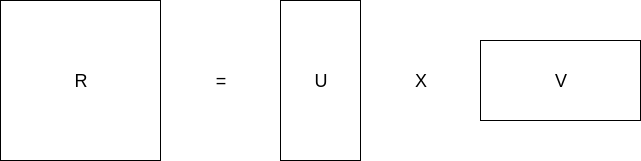
\includegraphics[width=\textwidth]{collaborative_filtering.png}
    \caption{Matrix Completion via Matrix Factorization}
    \label{fig:collaborative_filtering}
\end{figure}

In the Model-Based approach the problem is represented as a matrix completion problem.
The matrix $R$ in figure~\ref{fig:collaborative_filtering} represents the interactions of users and items, where $u_{ij}$ represents the interaction of user $i$ with item $j$.
Usually when dealing with such interaction data, this matrix is very sparse, since in general a user interacts with a small set out of possibly millions of items.
The main idea behind this approach is to fill in the missing entries of the matrix.
To achieve that we define two randomly initialized matrices $U$ and $V$ which when multiplied produce a matrix of the same shape as $U$.
As explained in~\cite{collaborative_filtering} these two matrices represent low rank representations of users and items respectively.
The next step is to use a optimization algorithm to fit $U$ and $V$ such that $r_{ij} \approx UV_{ij}$.
The error of the chosen optimization algorithm however is only applied to entries of $R$ which are known.
Therefore when we find $U$ and $V$ such that the values for the known entries match the values in $R$ we assume that we also found a good approximation for the values unkown in $R$ and use these to predict the interaction of the respective users and items.

\subsubsection{Often Bought Together}
Often/frequently bought together is a recommendation system very popular in online-stores.
The idea behind it is to recommend products that complement the one the user is intending to buy.
A classical example for this would be to recommend a protection case when the users adds a smartphone to the basket.
Therefore it is a item-based approach.
The implementation of this recommendation system can be done in a rather simple way, but can be improved a lot by complex systems, which could personalize the recommendations by using the users history, thereby extending it with a user-based component.
However the basic idea stays the same, as the name suggests, finding items that are frequently bought together.
The simplest, yet still effective, implementation of this is to just count how many times products appear in the same order as other products, i.e. for each combination of two products $i$ and $j$ we will have a count $c_{ij}$ of how many times these products were bought together.
When a user adds a product to the basket, we extract the products with the highest count from a database and recommend these to users.

\section{Concepts}
\subsection{Recurrent Neural Networks}\label{rnn}
Recurrent Neural Networks or RNNs are a form of artificial neural networks, which allow to explicitly model sequence input data.
The enabling factor for this is that RNNs allow the output of the network to be fed back in.

\begin{figure}[ht]
	\centering
	\captionsetup{width=0.8\textwidth}
    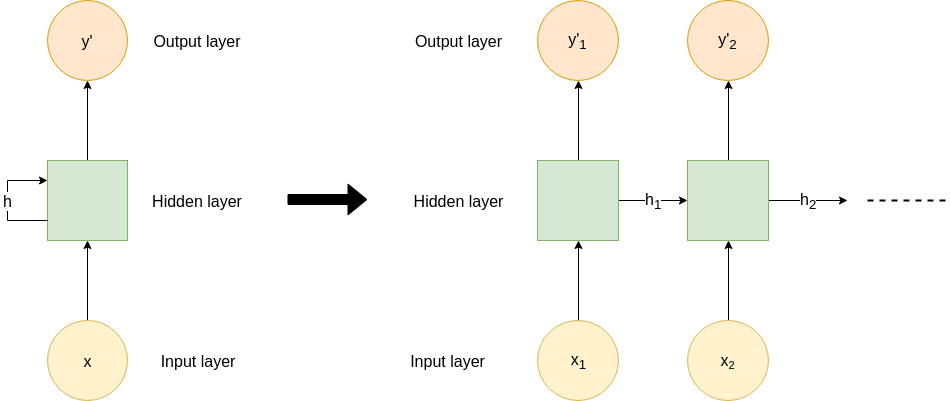
\includegraphics[width=\textwidth]{rnn.png}
    \caption{Recurrent Neural Network}
    \label{fig:rnn}
\end{figure}

Further RNNs carry a so called hidden state, which is propagated along the temporal axis.
The following two equations from~\cite{rnn_survey} describe the general behaviour of a simple RNN unit as illustrated in figure~\ref{fig:rnn}.
\begin{equation}\label{eq:rnn_hidden_state}
    h_{i+1} = \sigma(W^{hx}x_i + W^{hh}h_i + b_h)
\end{equation}
\begin{equation}\label{eq:rnn_output}
    y'_i = \text{softmax}(W^{yh}h_i + b_y)
\end{equation}
We can see in equation~\ref{eq:rnn_hidden_state} how the hidden state is carried over.
This equation represents the connections across the temporal axis mentioned above.
Figure~\ref{fig:rnn} shows how the sequence input denoted by $x$ is unfolded and fed into the network one timestep at a time.
For each timestep the corresponding output is computed as well as the hidden state that is carried over to the next timestep.
Intuitively the hidden state can be seen as the variable holding the relevant information from the previous steps to influence the prediction of the next step.
\par
For clarification purposes it is important to note that the individual inputs $x_t$ represent a datapoint in a sequence denoted by $x$, therefore in most cases are represented by a vector.
In a feedforward neural network as illustrated in figure~\ref{fig:ffnn}, the inputs $x_i$ represent individual entries in the feature vector of the datapoint $x$.
\subsubsection{Backpropagation}
Backpropagation is the technique used to train neural networks.

\begin{figure}[ht]
	\centering
	\captionsetup{width=0.8\textwidth}
    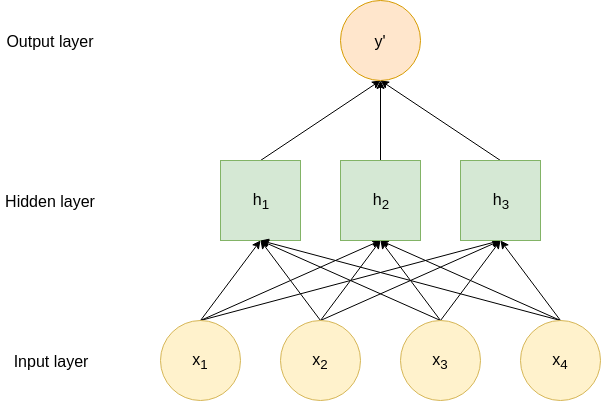
\includegraphics[width=0.8\textwidth]{ffnn.png}
    \caption{Feedforward Neural Network}
    \label{fig:ffnn}
\end{figure}

Let us assume we have a simple feedforward neural network as shown in figure~\ref{fig:ffnn}.
This behaviour of this network is described by the following equations.
\begin{equation}\label{eq:ffnn_hidden_layer}
    h_i = \sigma_h(w_{h_i}^Tx)
\end{equation}
\begin{equation}\label{eq:ffnn_output}
    y' = \sigma_y(w_{y}^Th)
\end{equation}
Each individual cell has a weight vector associated with it denoted by $w_o$ where $o$ is the respective cell.
The arrows in the illustration represent the individual weights of such a weight vector.
Further each layer has an nonlinear activation function associated with it, denoted by $\sigma_l$, $l$ being the respective layer.
\par
In this setting we usually are in a supervised mode, where for each input $x$ there is a true label $y$.
Using the neural network we estimate $y$ for a given $x$ by applying the equations above to obtain the estimation $y'$.
\par
The last component needed before training is possible is a loss function $\mathcal{L}(y, y')$, which quantifies the error of the estimation $y'$.
\par
The basic idea of backpropagation is to attribute parts of the error computed to the different units of the network, and therefore make adjustements to the weight vector of a particular unit.
As described in~\cite{rnn_survey} this is done by using the chain rule to compute the derivative of $\mathcal{L}(y, y')$ with respect to each weight vector.
The weight vector is then adjusted by gradient descent, i.e. by moving the vector in the direction of the largest decrease in the gradient.
There are more parameters involved such as the learning rate, which defines how much in the direction of the gradient the weights are adjusted, however these are not needed for understanding the principle.
\subsubsection{Backpropagation with RNNs}
Also in~\cite{rnn_survey} the authors mention that training RNNs has been known to be especially difficult due to the \emph{vanishing} or \emph{exploding gradients} problem.
As an example we consider the RNN in figure~\ref{fig:rnn}.
Now we assume we compute the estimation $y'_t$, i.e. the output of timestep $t$.
As we can see in the equations~\ref{eq:1} and~\ref{eq:rnn_output} this output is also influenced by all the previous timesteps.
The problem now arises from the so called recurrent weights denoted by $W^{hh}$, those connecting the units across the temporal axis.
For now we assume that the weights are small, i.e. $|w_{ij}| < 1$ for $w_{ij} \in W^{hh}$.
Since the weights are small, the contribution of input $x_{t-k}$ to the output $y'_t$ gets exponentially smaller with increasing $k$.
Essentially by computing the gradient with respect to the input the afromentioned contribution is quantified.
Therefore when $k$ gets large and the contribution of the input $x_{t-k}$ vanishes, the gradient with respect to the input unit also vanishes, resulting in the so called vanishing gradient problem.
The opposite happens when the recurrent weights are large, i.e. $|w_{ij}| > 1$ for $w_{ij} \in W^{hh}$.
In this case the contribution gets amplified when $k$ gets large, and therefore we would be dealing with exploding gradients.
This is a problem in a setting where we want to learn long-range dependencies, which is often the case in sequence modeling.

\subsubsection{Gated Recurrent Unit}
The Gated Recurrent Unit (GRU) is a recurrent unit which aims to solve the exploding or vanishing gradients problem mentioned above.
This is achieved by modifying the behaviour of the hidden units, in between which the recurrent edges of the network are.
The authors of~\cite{gru} introduced this new type of recurrent unit.
They retrofitted the recurrent unit with the ability to adaptively remember and forget.
This is achieved using two gates: The \emph{reset} and \emph{update} gate.
\par
The reset gate is responsible to supress features of the hidden state that were learned to be not important in the future.
The reset gate is computed using the following formula:
\begin{equation}\label{eq:gru_reset_gate}
    r_t = \sigma( W_rx + U_rh_{t-1} + b_r)
\end{equation}
The matrices $W_r$ and $U_r$ and the bias $b_r$ are parameters specific to the reset gate and are learned simultaneously with backpropagation.
\par
The update gate controls how much information is propagated from the previous hidden state to the next one, i.e. it learns which features of the previous hidden state will be how important in the future.
The update gate is computed as follows:
\begin{equation}\label{eq:gru_update_gate}
    z_t = \sigma( W_zx + U_zh_{t-1} + b_z)
\end{equation}
Again the weight matrices and bias are specific to the update gate and learned via backpropagation.
\par
To compute the next hidden state the computed gates are used as follows:
\begin{equation}\label{eq:gru_hidden_state}
    h_t = z_t \circ h_{t-1} + (1 - z_t) \circ \text{tanh}(W_hx_t + U_h(r_t \circ h_{t-1}) + b_h)
\end{equation}
In equation~\ref{eq:gru_hidden_state} we can see how the gates do their job.
When the reset gate is close to 0 in some features, the hidden state is forced to ignore that information before being multiplied with the weight matrix of the recurren unit.
On the other hand, the update gate controls how much information should be propagated directly from the hidden state, versus the hidden state resulting from the new input.
If the reset gate is 1 and the update gate is 0 we get the same formula as in~\ref{eq:rnn_hidden_state}, effectively returning to the vanilla RNN formulation.
\subsection{Embeddings of categorical variables}
A categorical variable is variable that can take one of a limited number of values.
Examples are colors, locations or, in the context of e-commerce, product ids.
When using such variables as an input variable for some model, the variables need to be transformed into a numerical representation, such that the variable can be used.
Let us assume we have a variable which describes the color of a specific product.
For simplicity we assume there are only four colors: red, green, blue, yellow.
One possibility would be to just assign integer ids to the different colors as shown in table~\ref{tab:id_encoding}.

\begin{table}[ht]
    \centering
    \begin{tabular}{c|c}
    Color & Id \\ \hline
    Red & 0 \\
    Green & 1 \\
    Blue & 2 \\
    Yellow & 3
    \end{tabular}
    \caption{Integer Ids for Colors}
    \label{tab:id_encoding}
\end{table}

The problem with this approach is that integers have a defined order.
That means that any model will interpret the color yellow as larger or as a stronger signal, than the color red.
This is not desirable, in the case of colors, all of them should have the same magnitude so to speak.
\par
A different way of representing categorical variables is the so called one-hot encoding.
A one-hot encoding requires a continuous id space, such as the one in table~\ref{tab:id_encoding}.
The same colors encoded in a one-hot encoding can be seen in table~\ref{tab:one_hot_encoding}.

\begin{table}[ht]
    \centering
    \begin{tabular}{c|c}
    Color & One-Hot Encoding \\ \hline
    Red & $[1,0,0,0]$ \\
    Green & $[0,1,0,0]$ \\
    Blue & $[0,0,1,0]$ \\
    Yellow & $[0,0,0,1]$
    \end{tabular}
    \caption{One-Hot Encoding for Colors}
    \label{tab:one_hot_encoding}
\end{table}
Now all the color representations have the same magnitude, therefore the model will get the same signal strength from each of the colors.
In principle we transform the id encoding to a one-hot encoding by using a zero vector of dimension $\max(\text{id})$ and set the element at the position $\text{id}-1$ to 1.
Therefore the one-hot encoding always has the same dimensionality as the number of categories.
There are still two major drawbacks to this approach.
As we will see in section~\ref{sec:dataset_properties} the number of categories for such a variable can range into the millions.
This means that the dimensionality of the single categorical feature can range into the millions, obviously this is not desirable, since high dimensionality leads to more difficulties in training and more computing resources needed to accomplish the training task.
The second drawback is that this representation does not account for the notion of similarity, i.e. red is as similar to blue as it is to yellow.
However it is known that green is a composition of blue and yellow, so intuitively green should be more similar to blue and yellow than to red.
\par
These two issues can be solved by using embeddings.
Embeddings are a low dimensional real numbered representation of a categorical variable.
Further similar variables will have similar vectors representing them.
The difficulty with embeddings is finding a process which produces the embeddings with the desired properties.
For a small number of variables it is possible to manually construct them.
In table~\ref{tab:embedding} we can see a lower dimensional representation of the same colors, however now the distance between green and yellow or blue is smaller than the one between green and red.
Further all the representations still have the same magnitude, therefore not triggering a stronger signal depending on the color.
\begin{table}[ht]
    \centering
    \begin{tabular}{c|c}
    Color & Embedding \\ \hline
    Red & $[1,0,0]$ \\
    Green & $[0,\sqrt{0.5},\sqrt{0.5}]$ \\
    Blue & $[0,1,0]$ \\
    Yellow & $[0,0,1]$
    \end{tabular}
    \caption{Possible Embedding for Colors}
    \label{tab:embedding}
\end{table}

\section{Previous Work}
\subsection{Meta-Prod2Vec}
\begin{itemize}
    \item This is a model that allows us to capture the semantic similarity between products
    \item The basic assumption behind word2vec is that words that appear in similar contexts are similar.
    \item This comes from linguistics?
    \item How to explain the formula?
    \item Show equation of word2vec
    \item To apply this to products we interpred products as words and sessions as sentences.
    \item Additionally we introduce the notion of side information, by instantiating the metadata in the same space, and modeling the relations between metadata
\end{itemize}
\cite{prod2vec}
\subsection{Hierarchical RNNs for personalized Recommendations}
\begin{itemize}
    \item This is the starting point for the thesis
    \item Which components does the system have?
    \item Show the graphic from the paper
\end{itemize}
\cite{hierarchical}

\section{KPIs}
\subsection{Click-Through-Rate}
\subsection{Conversion Rate}\label{conversion_rate}
\begin{itemize}
\item Describe different KPIs
\item What do they meaure, how to optimize for it
\end{itemize}